\documentclass[tikz,border=4pt]{standalone}
\usepackage[utf8]{inputenc}
\usepackage[T1]{fontenc}
\usetikzlibrary{positioning,arrows.meta,fit,backgrounds}
\definecolor{gcn}{HTML}{2a78d6}
\definecolor{base}{HTML}{eb6834}
\definecolor{tinta}{HTML}{52514e}
\definecolor{leve}{HTML}{f2f6fc}
\begin{document}
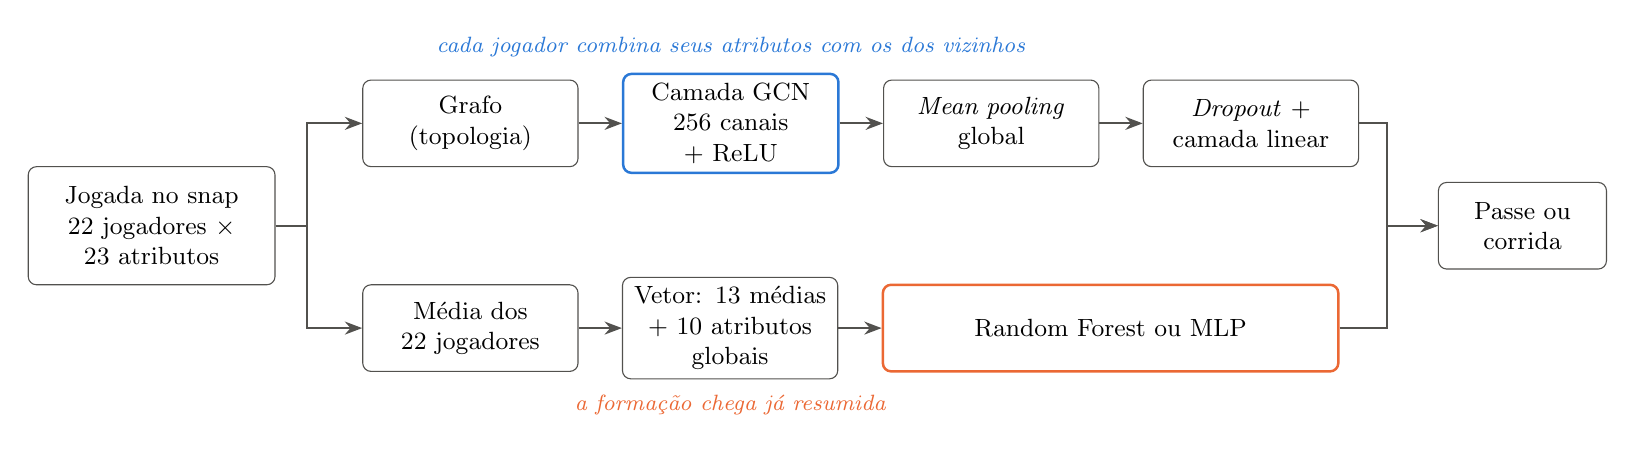
\begin{tikzpicture}[
  font=\small,
  caixa/.style={draw=tinta, rounded corners=3pt, align=center, minimum height=1.1cm, text width=2.5cm, fill=white},
  seta/.style={-{Stealth[length=2.2mm]}, thick, draw=tinta},
  node distance=0.5cm and 0.55cm]
% ---- entrada comum
\node[caixa, text width=2.9cm, minimum height=1.5cm] (x) {Jogada no snap\\22 jogadores $\times$\\23 atributos};
% ---- ramo GCN
\node[caixa, right=1.1cm of x, yshift=1.3cm] (g1) {Grafo\\(topologia)};
\node[caixa, right=of g1, draw=gcn, line width=0.9pt] (g2) {Camada GCN\\256 canais + ReLU};
\node[caixa, right=of g2] (g3) {\textit{Mean pooling}\\global};
\node[caixa, right=of g3] (g4) {\textit{Dropout} +\\camada linear};
% ---- ramo baselines
\node[caixa, right=1.1cm of x, yshift=-1.3cm] (b1) {M\'edia dos\\22 jogadores};
\node[caixa, right=of b1] (b2) {Vetor: 13 m\'edias\\+ 10 atributos\\globais};
\node[caixa, right=of b2, draw=base, line width=0.9pt, text width=5.55cm] (b3) {Random Forest ou MLP};
% ---- saida
\node[caixa, right=1.0cm of g4, yshift=-1.3cm, text width=1.9cm] (y) {Passe ou\\corrida};
\draw[seta] (x.east) -- ++(0.4,0) |- (g1.west);
\draw[seta] (x.east) -- ++(0.4,0) |- (b1.west);
\draw[seta] (g1) -- (g2); \draw[seta] (g2) -- (g3); \draw[seta] (g3) -- (g4);
\draw[seta] (b1) -- (b2); \draw[seta] (b2) -- (b3);
\draw[seta] (g4.east) -- ++(0.35,0) |- (y.west);
\draw[seta] (b3.east) -| ([xshift=0.35cm]g4.east |- y.west) -- (y.west);
\node[font=\footnotesize\itshape, text=gcn, above=0.08cm of g2] {cada jogador combina seus atributos com os dos vizinhos};
\node[font=\footnotesize\itshape, text=base, below=0.08cm of b2] {a forma\c{c}\~ao chega j\'a resumida};
\end{tikzpicture}
\end{document}
